%%%%%%%%%%%%%%%%%%%%%%%%%%%%%%%%%%%%%%%%%
% FRI Data Science_report LaTeX Template
% Version 1.0 (28/1/2020)
% 
% Jure Demšar (jure.demsar@fri.uni-lj.si)
%
% Based on MicromouseSymp article template by:
% Mathias Legrand (legrand.mathias@gmail.com) 
% With extensive modifications by:
% Antonio Valente (antonio.luis.valente@gmail.com)
%
% License:
% CC BY-NC-SA 3.0 (http://creativecommons.org/licenses/by-nc-sa/3.0/)
%
%%%%%%%%%%%%%%%%%%%%%%%%%%%%%%%%%%%%%%%%%


%----------------------------------------------------------------------------------------
%	PACKAGES AND OTHER DOCUMENT CONFIGURATIONS
%----------------------------------------------------------------------------------------
\documentclass[fleqn,moreauthors,10pt]{ds_report}
\usepackage[english]{babel}

\graphicspath{{fig/}}




%----------------------------------------------------------------------------------------
%	ARTICLE INFORMATION
%----------------------------------------------------------------------------------------

% Header
\JournalInfo{FRI Natural language processing course 2024}

% Interim or final report
\Archive{Project report} 
%\Archive{Final report} 

% Article title
\PaperTitle{Conversations with Characters in Stories for Literacy — Quick, Customized Persona Bots from novels} 

% Authors (student competitors) and their info
\Authors{Leon Todorov, Jan Rojc, Andraž Zrimšek}

% Advisors
\affiliation{\textit{Advisors: Slavko Žitnik}}

% Keywords
\Keywords{PersonaBots, In Context Learning, Large Language Models}
\newcommand{\keywordname}{Keywords}


%----------------------------------------------------------------------------------------
%	ABSTRACT
%----------------------------------------------------------------------------------------

\Abstract{
% There is a world-wide literacy crisis (\cite{doi:10.1080/09669760.2021.1883816}\cite{tue2014beyond}\cite{pisa2018}). Young people hate reading and rarely read recreationally. They fail at high level literacy skills, e.g., evaluating texts for validity and integrating across texts to create personal knowledge. Yet, literacy is vital for educational and professional success, life happiness and societal health. One way to motivate young people to read is through conversational interaction with digital personifications of characters (pedagogical agents or PersonaBots) in novels. LLMs provide possible solutions. Khanmigo offers personaBot ChatGPT text conversations with Jay Gatsby (of the classic novel, The Great Gatsby) and with Obama. However, their offerings are limited. Khanamigo provides no information on development time for personaBots, nor does it offer customized personaBots from user-suggested novels. Quick, customized personaBots, for conversations with characters, based on teacher-suggested novels would be enormously educational. To ensure a personaBot is fully contextualized in the specific context and at the same time within the constraints of token limitations, our suggestion is considering the current Retrieval and indexing techniques (i.e., Retrieval Augmented Generation) or implementing more efficient vector searching or similarity computation approaches.
This paper explores the design and potential of PersonaBots, digital personifications of characters, as a novel way to engage with literature. We address the challenges of creating PersonaBots from user-suggested novels due to the limited token count of character descriptions. Our approach includes the use of Large Language Models (LLMs), Retrieval-Augmented Generation (RAG), and In Context Learning (ICL). We also delve into the educational potential of PersonaBots, as pedagogical agents have shown promising results in enhancing children's learning. Furthermore, we explore the use of sentence comparison techniques and situation models to create a bot that responds in a way that is consistent with its backstory. The process of corpus analysis, where we extract books from The Project Gutenberg repository for our study, is also discussed. This comprehensive exploration of the theoretical systems informing PersonaBot design, the evaluation of pedagogical agents, and the existing services available for PersonaBot creation contributes to the ongoing discourse on the use of digital technologies in literature and education.
}
%----------------------------------------------------------------------------------------

\begin{document}

% Makes all text pages the same height
\flushbottom 

% Print the title and abstract box
\maketitle 

% Removes page numbering from the first page
\thispagestyle{empty} 

%----------------------------------------------------------------------------------------
%	ARTICLE CONTENTS
%----------------------------------------------------------------------------------------

\section*{Introduction}

% The advent of digital technologies has revolutionized many aspects of our lives, including how we interact with literary characters. PersonaBots, or digital personifications of characters, offer a novel way to engage with literature. These bots can be customized to mimic the personality and dialogue of characters from novels, thereby providing a unique and interactive reading experience.

% However, creating a personaBot from a character in a user-suggested novel can be challenging due to the limited token count of character descriptions. This paper aims to address this issue by exploring various approaches to personaBot design, including the use of Large Language Models (LLMs), Retrieval-Augmented Generation (RAG), and In Context Learning (ICL).

% We also delve into the educational potential of personaBots. Pedagogical agents have shown promising results in enhancing children's learning, improving both question-asking skills and vocabulary learning. By transforming these agents into text conversations with characters from novels, we aim to motivate users to read more and improve learning.

% Furthermore, we explore the use of sentence comparison techniques and situation models to create a bot that responds in a way that is consistent with its backstory. We also discuss the process of corpus analysis, where we extract books from The Project Gutenberg repository for our study.

% This paper presents a comprehensive exploration of the theoretical systems informing personaBot design, the evaluation of pedagogical agents, and the existing services available for personaBot creation. Our findings will contribute to the ongoing discourse on the use of digital technologies in literature and education.

Digital technologies have transformed our interaction with literary characters through PersonaBots. These bots, mimicking characters from novels, offer a unique reading experience. However, creating PersonaBots from user-suggested novels is challenging due to limited token count. This paper explores PersonaBot design using Large Language Models (LLMs), Retrieval-Augmented Generation (RAG), and In Context Learning (ICL).

We also investigate the educational potential of PersonaBots as pedagogical agents, which have shown to enhance children's learning. This is crucial considering the current worldwide literacy crisis. Existing services like Khanmigo offer limited PersonaBot conversations. We propose quick, customized PersonaBots based on teacher-suggested novels, considering current retrieval and indexing techniques.

Additionally, we explore sentence comparison techniques and situation models for bot backstory consistency and discuss corpus analysis using The Project Gutenberg repository. This paper contributes to the discourse on digital technologies in literature and education.


%------------------------------------------------

\section*{Related work}
% Existing services (on personaBots and pedagogical agents in language arts) - Leon \\
\textbf{Existing services} \\
There currently exist many customizable personaBot services, such as character.ai, chatfai.com, dreamtavern.ai, moemate.io and many others. Most just use a basic character description ("How would your character describe themselves?"), but some implementations are extended by adding exemplary character greetings/dialogue or by directly adding additional backstories (sometimes even from external sources). While these platforms offer customization, the character descriptions usually have a very limited token count, which might be problematic when trying to create a custom personaBot from a character in a user-suggested novel.\\
\textbf{Pedagogical agents evaluation} \\
Pedagogical agents show promising results for enhancing children's learning (\cite{DBLP:journals/corr/abs-2004-03472}\cite{doi:10.1177/0735633117708283}). They can improve both question-asking skills and vocabulary learning depending on the design of the agent and the students' characteristics, hence pedagogical agents in the form of text conversation with characters from novels might motivate its users to read more and improve learning. \\

\textbf{Theoretical systems informing PersonaBot design} \\
When looking at conversational AI systems, there are multiple approaches of that have been studied. The model proposed in \cite{papaioannou2022designing} takes a more rule-based approach, but is mostly made to retain a human's attention rather than mimic a personality. A more useful approach is considered in \cite{li2016persona}, where a character is represented by an embedding, which should be close to the embeddings of words that are commonly around the character. With the rise of large language models (LLMs), \cite{minaee2024large} which perform great with conversational tasks, we are given many pre-trained models that can be considered. They perform great on general topics but require additional information when adapting to a specific domain. For this, we require the use of Retrieval-Augmented Generation (RAG). They allow us to find information relevant to the task from outside sources. This information can then be added to the language model's context using In Context Learning. LLMs, in combination with ICL, represent a possible approach to mimicking a persona without any parameter updates. For ICL an open source toolkit OpenICL \cite{wu2023openicl} has been released, which offers state-of-the-art retrieval and inference methods that can use to adapt ICL to a specific problem. 

% --- Sentance comparison \\ tole pomojem zdele ni treba k bo sam prevec pa ni dost relevantno

\textbf{Sentence comparison} 
When looking at comparing sentences, a good approach is embedding the sentence and using the spatial relation of sentence embeddings to find the closest ones. If only working with English sentences, \cite{reimers-gurevych-2019-sentence} offers a sentence embedding model based on a pretrained BERT network. If we want to enable conversations with our model in multiple languages, using a language-agnostic sentence embedding model like LASER, presented in \cite{schwenk2017learning} offers a good solution.

\textbf{Situation models} \\
Situation models are mental representations built by readers to understand the characters, events, and overall setting described in the text. Zwaan et al. (1998) \cite{zwaan1998constructing} investigated which aspects of a situation model are actively monitored during reading. Their findings suggest that readers primarily focus on dimensions like time, causality, goals, and the protagonist. By incorporating these aspects of situation models into personaBots, we can create a bot that responds in a way that is consistent with its backstory.


\textbf{Corpus analysis} \\
In this project, we will be extracting books from The Project Gutenberg repository \cite{gutenberg} to serve as the text source for our analysis. The corpus consists of over 70,000 free eBooks. It focuses on older works whose copyright has expired in the United States, making them part of the public domain.

\section{Proposed solution}
The solution we propose is using ICL to help a pre-trained LLM produce answers that would relate to the character. The data we would use to give it context could be using question-answer pairs that will be automatically generated from the desired novel. A possible approach is proposed in \cite{mo_2023}. An efficient method for finding relevant questions would be to use quick vector comparison methods to compare the question with questions in our dataset and use the question-answer pairs as examples to add to our model's context.

\section{Methods}
At the core of our conversational agent lies a pre-trained LLaMA2 chat model. We provide it instructions through a carefully crafted system prompt, which essentially tells the LLaMA2 model how to behave and what information to consider when crafting responses.
\subsection{RAG}
To improve the performance of our conversational agent, we employ two types of RAG. To better capture the style of speaking of the character, we search the book for relevant lines spoken by the character. To better capture the context for the answer, we also search the entire book segments for the most relevant parts.
\subsubsection*{Sentence extraction}
When starting our model, we save the entire book into a class and extract lines spoken for each character. When the model receives a question, it embeds it using the \textit{multi-qa-mpnet-base-cos-v1} sentence transformer, which was trained for semantic search, especially for question-answer sentence pairs. It also returns normalized embeddings with length 1, which allows for easier comparison. With this, we aim to find the lines from our character that could be a response to the question. We compare the embedding to embeddings of all character lines and return the ones that are most similar according to cosine similarity.
\subsubsection*{Context extraction}
When importing the book, we also split the entire text into segments of length 500. When we receive a question, we also embed it using the \textit{all-mpnet-base-v2} sentence transformer and compare it to all the extracted segments. We add the two most similar to our prompt for context.
\subsubsection*{ICL}
The end product is a prompt which includes a system prompt telling our agent how to act, as well as top \textit{n} character lines and extracted context from the book.
\subsection{Evaluation}
\subsubsection*{Contextual awareness}
We can assess the conversational agent's ability to understand context by measuring its performance on questions that require using the surrounding information. Here, we propose several methods for obtaining context-dependent question-answer pairs:
\begin{itemize}
    \item Utilize a pre-trained model like mojians/E2E-QA-Mining to automatically extract question-answer pairs directly from the book. 
    \item Prompt LLM to generate follow-up questions based on a provided passage.
    \item Carefully select context-dependent questions from educational websites or other curated online sources.
    \item Manually craft context-dependent questions that specifically target the character's knowledge, experiences, or the overall story.
\end{itemize}
Now the context evaluation question and answer embeddings are extracted using the \textit{all-mpnet-base-v2} sentence transformer. Then we prompt the conversational agent with the question and compare the output embedding with the known answer's embedding.

\subsubsection*{Character personality}
We can evaluate how well the agent captures the character's personality by examining its responses to general conversational questions that don't necessarily have a specific answer in the book. These questions can be obtained by:
\begin{itemize}
    \item We can prompt LLM to generate open-ended questions.
    \item Manually crafting open-ended questions.
\end{itemize}

Now the personality evaluation question embeddings are extracted using the \textit{all-mpnet-base-v2} sentence transformer. For each extracted question the most relevant character line is extracted by comparing the question's embedding with the embeddings of all extracted character lines and selecting the one with the highest cosine similarity. Then we prompt the conversational agent with the question and compare the output embedding with the embedding of the most relevant character line.



% Use the Methods section to describe what you did an how you did it -- in what way did you prepare the data, what algorithms did you use, how did you test various solutions ... Provide all the required details for a reproduction of your work.

% Below are \LaTeX examples of some common elements that you will probably need when writing your report (e.g. figures, equations, lists, code examples ...).


% \subsection*{Equations}

% You can write equations inline, e.g. $\cos\pi=-1$, $E = m \cdot c^2$ and $\alpha$, or you can include them as separate objects. The Bayes’s rule is stated mathematically as:

% \begin{equation}
% 	P(A|B) = \frac{P(B|A)P(A)}{P(B)},
% 	\label{eq:bayes}
% \end{equation}

% where $A$ and $B$ are some events. You can also reference it -- the equation \ref{eq:bayes} describes the Bayes's rule.

% \subsection*{Lists}

% We can insert numbered and bullet lists:

% % the [noitemsep] option makes the list more compact
% \begin{enumerate}[noitemsep] 
% 	\item First item in the list.
% 	\item Second item in the list.
% 	\item Third item in the list.
% \end{enumerate}

% \begin{itemize}[noitemsep] 
% 	\item First item in the list.
% 	\item Second item in the list.
% 	\item Third item in the list.
% \end{itemize}

% We can use the description environment to define or describe key terms and phrases.

% \begin{description}
% 	\item[Word] What is a word?.
% 	\item[Concept] What is a concept?
% 	\item[Idea] What is an idea?
% \end{description}


% \subsection*{Random text}

% This text is inserted only to make this template look more like a proper report. Lorem ipsum dolor sit amet, consectetur adipiscing elit. Etiam blandit dictum facilisis. Lorem ipsum dolor sit amet, consectetur adipiscing elit. Interdum et malesuada fames ac ante ipsum primis in faucibus. Etiam convallis tellus velit, quis ornare ipsum aliquam id. Maecenas tempus mauris sit amet libero elementum eleifend. Nulla nunc orci, consectetur non consequat ac, consequat non nisl. Aenean vitae dui nec ex fringilla malesuada. Proin elit libero, faucibus eget neque quis, condimentum laoreet urna. Etiam at nunc quis felis pulvinar dignissim. Phasellus turpis turpis, vestibulum eget imperdiet in, molestie eget neque. Curabitur quis ante sed nunc varius dictum non quis nisl. Donec nec lobortis velit. Ut cursus, libero efficitur dictum imperdiet, odio mi fermentum dui, id vulputate metus velit sit amet risus. Nulla vel volutpat elit. Mauris ex erat, pulvinar ac accumsan sit amet, ultrices sit amet turpis.

% Phasellus in ligula nunc. Vivamus sem lorem, malesuada sed pretium quis, varius convallis lectus. Quisque in risus nec lectus lobortis gravida non a sem. Quisque et vestibulum sem, vel mollis dolor. Nullam ante ex, scelerisque ac efficitur vel, rhoncus quis lectus. Pellentesque scelerisque efficitur purus in faucibus. Maecenas vestibulum vulputate nisl sed vestibulum. Nullam varius turpis in hendrerit posuere.


% \subsection*{Figures}

% You can insert figures that span over the whole page, or over just a single column. The first one, \figurename~\ref{fig:column}, is an example of a figure that spans only across one of the two columns in the report.

% \begin{figure}[ht]\centering
% 	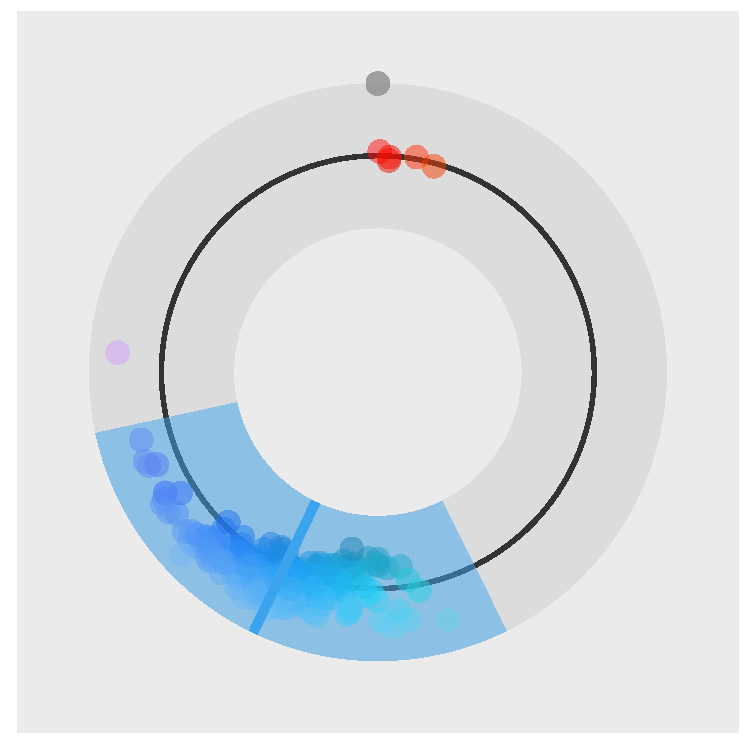
\includegraphics[width=\linewidth]{single_column.pdf}
% 	\caption{\textbf{A random visualization.} This is an example of a figure that spans only across one of the two columns.}
% 	\label{fig:column}
% \end{figure}

% On the other hand, \figurename~\ref{fig:whole} is an example of a figure that spans across the whole page (across both columns) of the report.

% % \begin{figure*} makes the figure take up the entire width of the page
% \begin{figure*}[ht]\centering 
% 	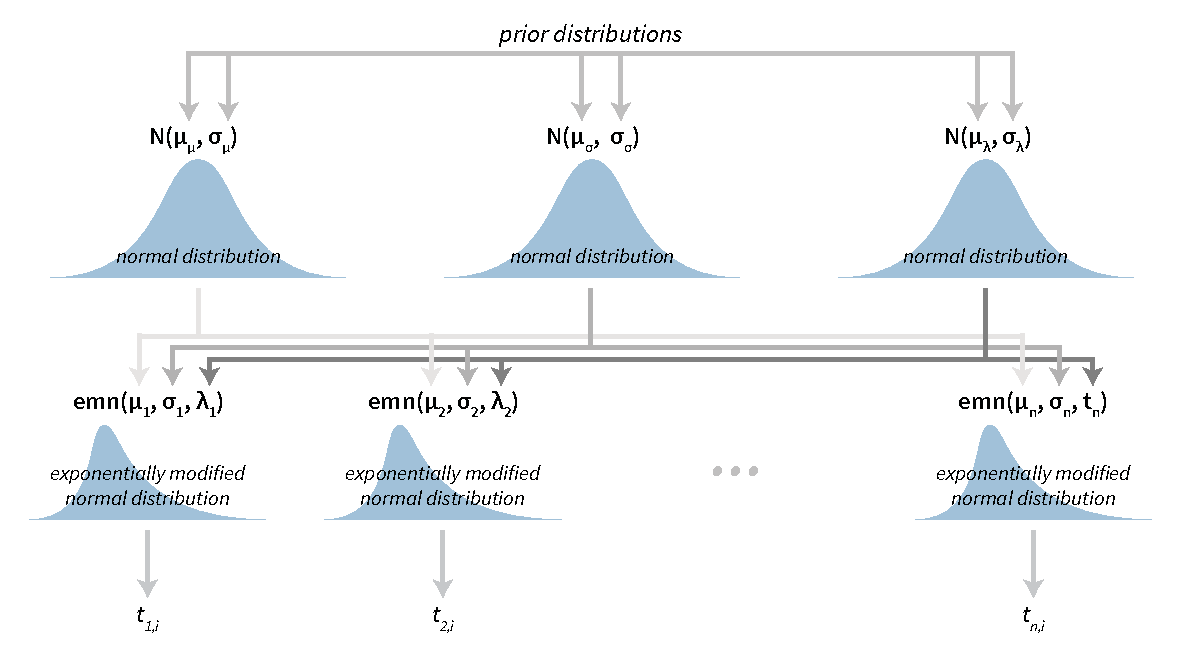
\includegraphics[width=\linewidth]{whole_page.pdf}
% 	\caption{\textbf{Visualization of a Bayesian hierarchical model.} This is an example of a figure that spans the whole width of the report.}
% 	\label{fig:whole}
% \end{figure*}


% \subsection*{Tables}

% Use the table environment to insert tables.

% \begin{table}[hbt]
% 	\caption{Table of grades.}
% 	\centering
% 	\begin{tabular}{l l | r}
% 		\toprule
% 		\multicolumn{2}{c}{Name} \\
% 		\cmidrule(r){1-2}
% 		First name & Last Name & Grade \\
% 		\midrule
% 		John & Doe & $7.5$ \\
% 		Jane & Doe & $10$ \\
% 		Mike & Smith & $8$ \\
% 		\bottomrule
% 	\end{tabular}
% 	\label{tab:label}
% \end{table}


% \subsection*{Code examples}

% You can also insert short code examples. You can specify them manually, or insert a whole file with code. Please avoid inserting long code snippets, advisors will have access to your repositories and can take a look at your code there. If necessary, you can use this technique to insert code (or pseudo code) of short algorithms that are crucial for the understanding of the manuscript.

% \lstset{language=Python}
% \lstset{caption={Insert code directly from a file.}}
% \lstset{label={lst:code_file}}
% \lstinputlisting[language=Python]{code/example.py}

% \lstset{language=R}
% \lstset{caption={Write the code you want to insert.}}
% \lstset{label={lst:code_direct}}
% \begin{lstlisting}
% import(dplyr)
% import(ggplot)

% ggplot(diamonds,
% 	   aes(x=carat, y=price, color=cut)) +
%   geom_point() +
%   geom_smooth()
% \end{lstlisting}

% %------------------------------------------------

% \section*{Results}

% Use the results section to present the final results of your work. Present the results in a objective and scientific fashion. Use visualisations to convey your results in a clear and efficient manner. When comparing results between various techniques use appropriate statistical methodology.

% \subsection*{More random text}

% This text is inserted only to make this template look more like a proper report. Lorem ipsum dolor sit amet, consectetur adipiscing elit. Etiam blandit dictum facilisis. Lorem ipsum dolor sit amet, consectetur adipiscing elit. Interdum et malesuada fames ac ante ipsum primis in faucibus. Etiam convallis tellus velit, quis ornare ipsum aliquam id. Maecenas tempus mauris sit amet libero elementum eleifend. Nulla nunc orci, consectetur non consequat ac, consequat non nisl. Aenean vitae dui nec ex fringilla malesuada. Proin elit libero, faucibus eget neque quis, condimentum laoreet urna. Etiam at nunc quis felis pulvinar dignissim. Phasellus turpis turpis, vestibulum eget imperdiet in, molestie eget neque. Curabitur quis ante sed nunc varius dictum non quis nisl. Donec nec lobortis velit. Ut cursus, libero efficitur dictum imperdiet, odio mi fermentum dui, id vulputate metus velit sit amet risus. Nulla vel volutpat elit. Mauris ex erat, pulvinar ac accumsan sit amet, ultrices sit amet turpis.

% Phasellus in ligula nunc. Vivamus sem lorem, malesuada sed pretium quis, varius convallis lectus. Quisque in risus nec lectus lobortis gravida non a sem. Quisque et vestibulum sem, vel mollis dolor. Nullam ante ex, scelerisque ac efficitur vel, rhoncus quis lectus. Pellentesque scelerisque efficitur purus in faucibus. Maecenas vestibulum vulputate nisl sed vestibulum. Nullam varius turpis in hendrerit posuere.

% Nulla rhoncus tortor eget ipsum commodo lacinia sit amet eu urna. Cras maximus leo mauris, ac congue eros sollicitudin ac. Integer vel erat varius, scelerisque orci eu, tristique purus. Proin id leo quis ante pharetra suscipit et non magna. Morbi in volutpat erat. Vivamus sit amet libero eu lacus pulvinar pharetra sed at felis. Vivamus non nibh a orci viverra rhoncus sit amet ullamcorper sem. Ut nec tempor dui. Aliquam convallis vitae nisi ac volutpat. Nam accumsan, erat eget faucibus commodo, ligula dui cursus nisi, at laoreet odio augue id eros. Curabitur quis tellus eget nunc ornare auctor.


% %------------------------------------------------

% \section*{Discussion}

% Use the Discussion section to objectively evaluate your work, do not just put praise on everything you did, be critical and exposes flaws and weaknesses of your solution. You can also explain what you would do differently if you would be able to start again and what upgrades could be done on the project in the future.


% %------------------------------------------------

% \section*{Acknowledgments}

% Here you can thank other persons (advisors, colleagues ...) that contributed to the successful completion of your project.


%----------------------------------------------------------------------------------------
%	REFERENCE LIST
%----------------------------------------------------------------------------------------
\bibliographystyle{unsrt}
\bibliography{report}
\end{document}